\documentclass[11pt]{article}
\usepackage{geometry}                % See geometry.pdf to learn the layout options. There are lots.
\geometry{letterpaper}                   % ... or a4paper or a5paper or ... 
%\geometry{landscape}                % Activate for for rotated page geometry
%\usepackage[parfill]{parskip}    % Activate to begin paragraphs with an empty line rather than an indent
\usepackage{graphicx}
\usepackage{amssymb}
\usepackage{epstopdf}
\DeclareGraphicsRule{.tif}{png}{.png}{`convert #1 `dirname #1`/`basename #1 .tif`.png}

%

\usepackage[nottoc]{tocbibind} %for table of contents
\usepackage{amsmath}
\usepackage{wrapfig}
\usepackage{caption}
\usepackage{subcaption}
\usepackage{verbatim} %for multiline comments
\usepackage{ulem}

\title{Computational Physics Project A \\ Modelling Single \& Double Pendulum Systems Computationally}
\author{Joshua Maxey}
%\date{}                                           % Activate to display a given date or no date

\begin{document}
\maketitle

\begin{center}
\begin{it}
The Euler, Leapfrog and 4th order Runge-Kutta (RK4) numerical methods are used to computationally model a single pendulum system in C++. By varying system and method parameters limits are found for the stabiity of these methods and their suitability for oscillatory problems. The conclusions of this preliminary investigation feed into simulating the more complex double pendulum system, deriving an understanding of the motion and movement of energy between the pudulums as well as finding limits of applicability of the RK4 for this system.
\end{it}
\end{center}

\tableofcontents
\pagebreak

\section{Introduction}
Computational models of physical systems require us to discretise continuous variables (often, but not exclusively, time). Numerical methods approximate derivatives to provide a means to solving differential equaitons computationally. The three numerical methods investigated in this project are Euler's method, the Leapfrog method and the 4th order Runge-Kutta method.

\begin{comment}

                                                                                          
          88                         88                                                   
          ""                         88                                                   
                                     88                                                   
,adPPYba, 88 8b,dPPYba,   ,adPPYb,d8 88  ,adPPYba,    8b,dPPYba,   ,adPPYba, 8b,dPPYba,   
I8[    "" 88 88P'   `"8a a8"    `Y88 88 a8P_____88    88P'    "8a a8P_____88 88P'   `"8a  
 `"Y8ba,  88 88       88 8b       88 88 8PP"""""""    88       d8 8PP""""""" 88       88  
aa    ]8I 88 88       88 "8a,   ,d88 88 "8b,   ,aa    88b,   ,a8" "8b,   ,aa 88       88  
`"YbbdP"' 88 88       88  `"YbbdP"Y8 88  `"Ybbd8"'    88`YbbdP"'   `"Ybbd8"' 88       88  
                          aa,    ,88                  88                                  
                           "Y8bbdP"                   88                                  

\end{comment}

\section{The Single Pendulum}
\subsection{Theory}
\subsubsection*{System Description \& Parameters}
The idealised single pendulum system comprises a fixed mass $m$ attached to the end of a massless rod of length $l$ suspended from a pivot which applies a friction that is characterised by the damping constant $\gamma$. It is depicted in figure \ref{fig:pendulum_diag} (a).

\begin{figure}[h]
	\begin{center}
		\includegraphics[width=0.5\textwidth]{img/sp_dp_diag.png}
		\caption{The single \& double pendulum notation used throughout this investigation.}
		\label{fig:pendulum_diag}
	\end{center}
\end{figure}

\subsubsection*{Equations of Motion}
The motion of the pendulum is defined by equation \ref{eq:eom_sp} where $\theta$ is the angle the pendulum makes with the vertical.

\begin{equation} \label{eq:eom_sp}
	ml\frac{d^2 \theta}{dt^2} = -mg\sin(\theta) - \gamma\frac{d\theta}{dt}
\end{equation}

By applying the small angle approximation, choosing dimensionless units of time to yeild reduced time, $\widetilde{t}$, such that

\begin{equation} \label{eq:const_def}
	\widetilde{t} = t\sqrt{\frac{l}{g}} \;\;\; \text{and choosing} \;\;\; \beta = \frac{\gamma}{m \sqrt{gl}}
\end{equation}

equation \ref{eq:eom_sp} reduces to

\begin{equation} \label{eq:eomsp_reduced}
	\frac{d^2 \theta}{d\widetilde{t}^2} = \theta - \beta\frac{d\theta}{d\widetilde{t}}
\end{equation}

\begin{it}
(Note that throughout the rest of this report, all time is in units of this reduced, dimensionless, time and damping will be discussed in terms of $\beta$.)
\end{it}

Equation \ref{eq:eomsp_reduced} can be expressed as a pair of coupled first order differential equations where $\omega$ is the rate of change of $\theta$ with respect to reduced time. They are presented in equation \ref{eq:coupled_1_order}.

\begin{equation} \label{eq:coupled_1_order}
	\frac{d}{d\widetilde{t}} \begin{pmatrix}\theta \\ \omega \end{pmatrix} = \begin{pmatrix} 0 & 1 \\ -1 & -\beta \end{pmatrix} \begin{pmatrix}\theta \\ \omega \end{pmatrix}
\end{equation}

The kinetic and potential energy formulae for the single pendulum were approximated using the small angle approximation. They reduce to equations \ref{eq:sp_ke} and \ref{eq:sp_pe}. Only being concerned with energy ratios, the constants were omitted when these were implemented in code.

\begin{equation} \label{eq:sp_ke}
T = \frac{1}{2}ml^2\omega^2
\end{equation}

\begin{equation} \label{eq:sp_pe}
U = \frac{1}{2}mgl\theta^2
\end{equation}

\subsubsection*{A Computer Model for the Single Pendulum System}
\subsubsection*{Euler's Method}
Euler's method is the simplest numerical method employed. It is obtained by Taylor expanding our function at an advanced time step $t$ + $h$ and truncating the result after the first two terms. As such, it is accurate to $O(h^2)$. 

Defining $\uuline{L}$ as the 2x2 matrix from \ref{eq:coupled_1_order} we can create the update matrix \uuline{$T$} where $\uuline{T}$ is defined as $\uuline{I}$ + $h$ $\uuline{L}$. To apply Euler's method we simply multiply the position vector at the current time step by this update matrix to find the values of $\theta$ and $\omega$ at the next time step. Hence,

\begin{equation} \label{eq:euler_seperate}
	\begin{split}
		\theta_{n+1} &= \theta_{n} + h\omega_{n} \\
		\omega_{n+1} &= -h\theta_{n} + (1 -h \beta)\omega_{n}
	\end{split}
\end{equation}

\subsubsection*{The Leapfrog Method}
The Leapfrog method is the simplest finite difference method that requires the storing of system variables at a previous timestep. It produces a gradient estimate from $y_{n-1}$ and $y_{n}$ which it uses to calculate $y_{n+1}$.  Using our notation, the Leapfrog method can be expressed as

\begin{equation} \label{eq:lf_vector}
	\begin{pmatrix}\theta_{n+1} \\ \omega_{n+1} \end{pmatrix} = \begin{pmatrix}\theta_{n-1} \\ \omega_{n-1} \end{pmatrix} + 2 h \uuline{L} \begin{pmatrix}\theta_{n} \\ \omega_{n} \end{pmatrix}
\end{equation}
	These are manifest in code as equations \ref{eq:lf_seperate}
\begin{equation} \label{eq:lf_seperate}
	\begin{split}
		\theta_{n+1} &= \theta_{n-1} + 2h\omega_{n} \\
		\omega_{n+1} &= \omega_{n-1} - 2h( \theta_{n} + \beta \omega_{n} )
	\end{split}
\end{equation}

\subsubsection*{4th Order Runge-Kutta Method}
The Runge-Kutta method provide a generalisation for taking any number of gradients and producing a weighted average of them to predict the next value of $y$. This investigation employs the 4th order Runge-Kutta method (RK4). It is the highest order (and therefore most accurate) Runge-Kutta method where the number of evaulations required per step is less than or equal to the order of error. It is fourth order accurate; $O(h^4)$.

Although it requires significantly more evaluations per time step, the RK4 method is more computationally efficient due to its ability to remain accurate for much larger values of $h$. The set of equations \ref{eq:rk4_vector} show the four evaluations required before one can calculate the variables at the next time step.

\begin{equation} \label{eq:rk4_vector}
	\begin{split}
		\underline{k}_{1} &= h \uuline{L} \cdot \underline{y}_{n}  \\
		\underline{k}_{2} &= h \uuline{L} \cdot ( \underline{y}_{n} + \frac{1}{2} \underline{k}_{1}) \\
		\underline{k}_{3} &= h \uuline{L} \cdot ( \underline{y}_{n} + \frac{1}{2} \underline{k}_{2}) \\
		\underline{k}_{4} &= h \uuline{L} \cdot ( \underline{y}_{n} + \underline{k}_{3}) \\
		\underline{y}_{n+1} &= \underline{y}_{n} + \frac{1}{6} ( \underline{k}_{1} + 2\underline{k}_{2} + 2\underline{k}_{3} + \underline{k}_{4}) \\
		\text{where} \;\;\;\; \underline{y}_{n} &= \begin{pmatrix}\theta_{n} \\ \omega_{n} \end{pmatrix}
	\end{split}
\end{equation}

\subsection{Aims \& Method}
The preliminary investigation sought to determine the scope of application for the three numerical methods in question, as applied to the single pendulum system with a view to recommending the most appropriate method for more general and complex oscillatory problems. The motion was modelled for 100 seconds at a step size of $h$ = 0.01 for two values of $\beta$; the undamped $\beta$ = 0 case and the lightly damped $\beta$ = 0.2 case. In both cases $\theta_{initial}$ = 0.1 and $\omega_{initial}$ = 0. The pendulum's motion over time ($\theta$ vs $\widetilde{t}$ \space) are presented in figures \ref{fig:sp_beta0} \& \ref{fig:sp_beta0.2} respectively.

A stability test was also devised to determine the step size value at which each method became unstable. This required simulating the zero and lightly damped single pendulum using each of the methods for a range of step sizes (0.01 \textless $h$ \textless \space 4.0, incrementing $h$ by 0.01 each time) and finding the ratio of final energy to initial energy, $E_{ratio}$ in each case. For the undamped case, $E_{final}$ was expected to equal $E_{initial}$ as there was no simulated means for energy to leave or enter the system. Hence, plotting $E_{ratio}$ against increasing $h$ would allow us to see at what point each method became unstable. The dataset was analysed to obtain the value of $h$ at which $E_{ratio}$ began to lay out of the range 0.9 \textless \space $E_{ratio}$ \textless 1.1 for the zero damped case. In the lightly damped case, a similar condition was applied. A method was declared unstable when 0.9 $E_{ratio_{prev}}$  \textless \space $E_{ratio}$ \textless 1.1 $E_{ratio_{prev}}$ ie when $E_{ratio}$ differed from the previoud value by more that 10\%. Table \ref{tab:sp_stability} records the largest step size for which the simulation could be said to be stable in each case.

\subsection{Results \& Discussion}

Figure \ref{fig:sp_beta0} clearly shows that for an undamped pendulum, the Euler method is unstable as the amplitude of oscillation steadily grows over time while both Leapfrog and RK4 provide stable oscillating solutions in line with the physics we expect to observe.

Conversely, figure \ref{fig:sp_beta0.2} shows that Euler is stable for damped oscillating systems (a conclusion confirmed by running further steps with varying $\beta$ values). Leapfrog decays initially inline with expectations but as the amplitude oscillation approaches zero it becomes unstable and produces unrealistic solutions.

Throughout both simulations the forth order Runge-Kutta method produces sensible solutions inline with what we would expect, maintaining a constant oscillation amplitube in the undamped case and exhibiting a decaying amplitude in the lightly damped case.


\begin{figure}[h!] \label{fig:sp_motion}
  \centering
  \begin{subfigure}[h]{0.5\textwidth}
    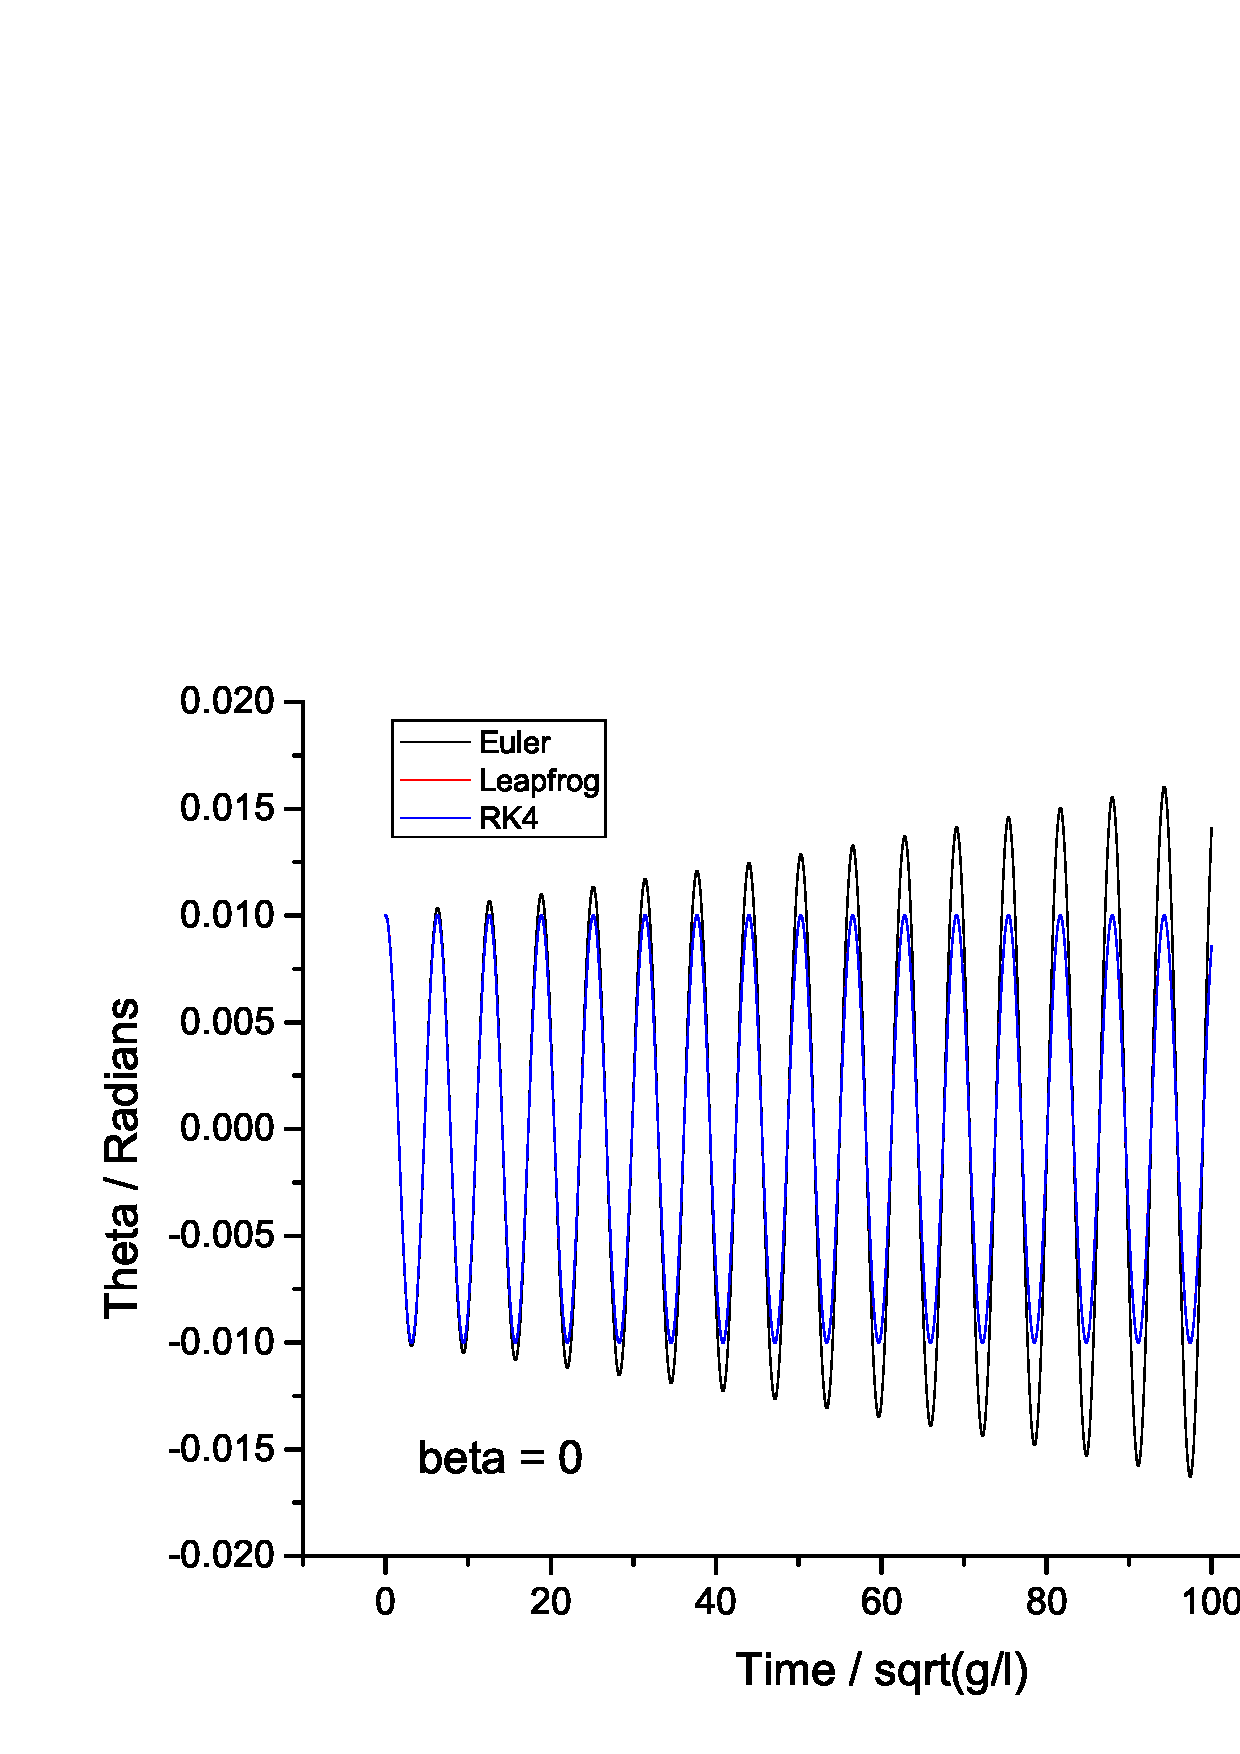
\includegraphics[width=\textwidth]{img/theta_vs_t_gamma=0.png}
    \captionsetup{width=0.85\textwidth}
    \caption{The motion of the single pedulum over time for the zero damping case ($\beta$ = 0). While the leapfrog data is present, it aggrees so strongly with the RK4 data that it's red line is obscured in this plot}
    \label{fig:sp_beta0}
  \end{subfigure}%
  ~ %add desired spacing between images, e. g. ~, \quad, \qquad etc.
    %(or a blank line to force the subfigure onto a new line)
  \begin{subfigure}[h]{0.5\textwidth}
    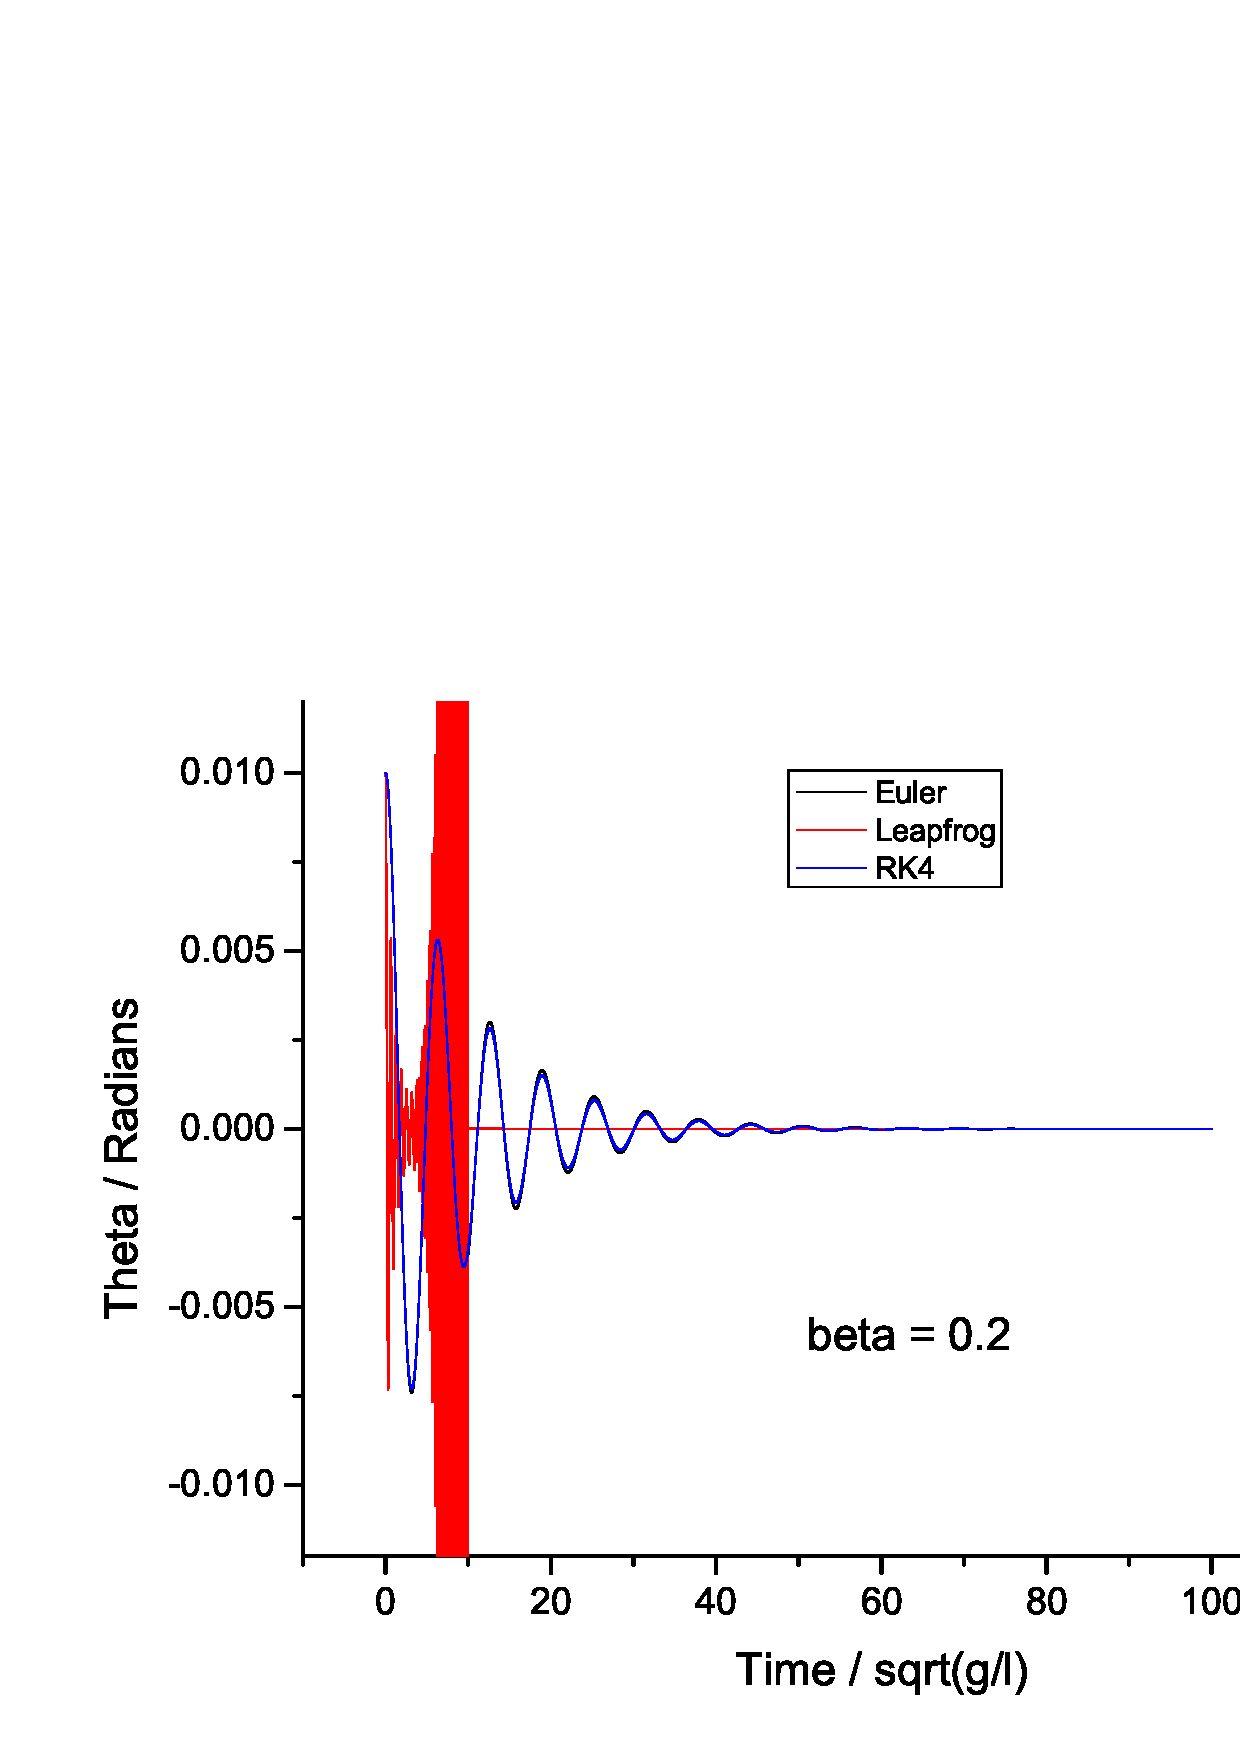
\includegraphics[width=\textwidth]{img/theta_vs_t_gamma=0-2.png}
    \captionsetup{width=0.85\textwidth}
    \caption{The motion of the single pedulum over time for the light damping case ($\beta$ = 0.2)}
    \label{fig:sp_beta0.2}
  \end{subfigure}
  \caption{The motion of the single pedulum as modelled by the three different numerical methods for zero and slight damping. In both cases the simulation ran for 100s with $h$ = 0.01.}
\end{figure}

Plotting $E_{ratio}$ against increasing $h$ for each method, both damped and undamped (figure \ref{e_vs_h}), summarises our stability and applicability findings concisely. It is clear to see that Euler is only stable for relatively small values of $h$ and only applicable for damped oscillatory problems.

Leapfrog is only applicable in the undamped scenario, as made clear by figure \ref{fig:sp_motion}. Figure \ref{e_vs_h} shows that it is second quickest to become unstable, producing erratic results from $h$ \textgreater 0.36 onwards.

Lastly, the forth order Runge-Kutta method remains stable for zero and non-zero $\beta$ values. In the damped case, while $E_{ratio}$ starts to deviate from 1 at around $h$ \= 0.57 (the point at which $E_{ratio}$ \textless 0.9), the results remain stable for much larger $h$ values than the other two methods. This suggests that while these larger step sizes do not cause the simulation to break down entirely, the error in results may become significant. The exact nature of this error is beyond the scope of this investigation.

\begin{figure}
	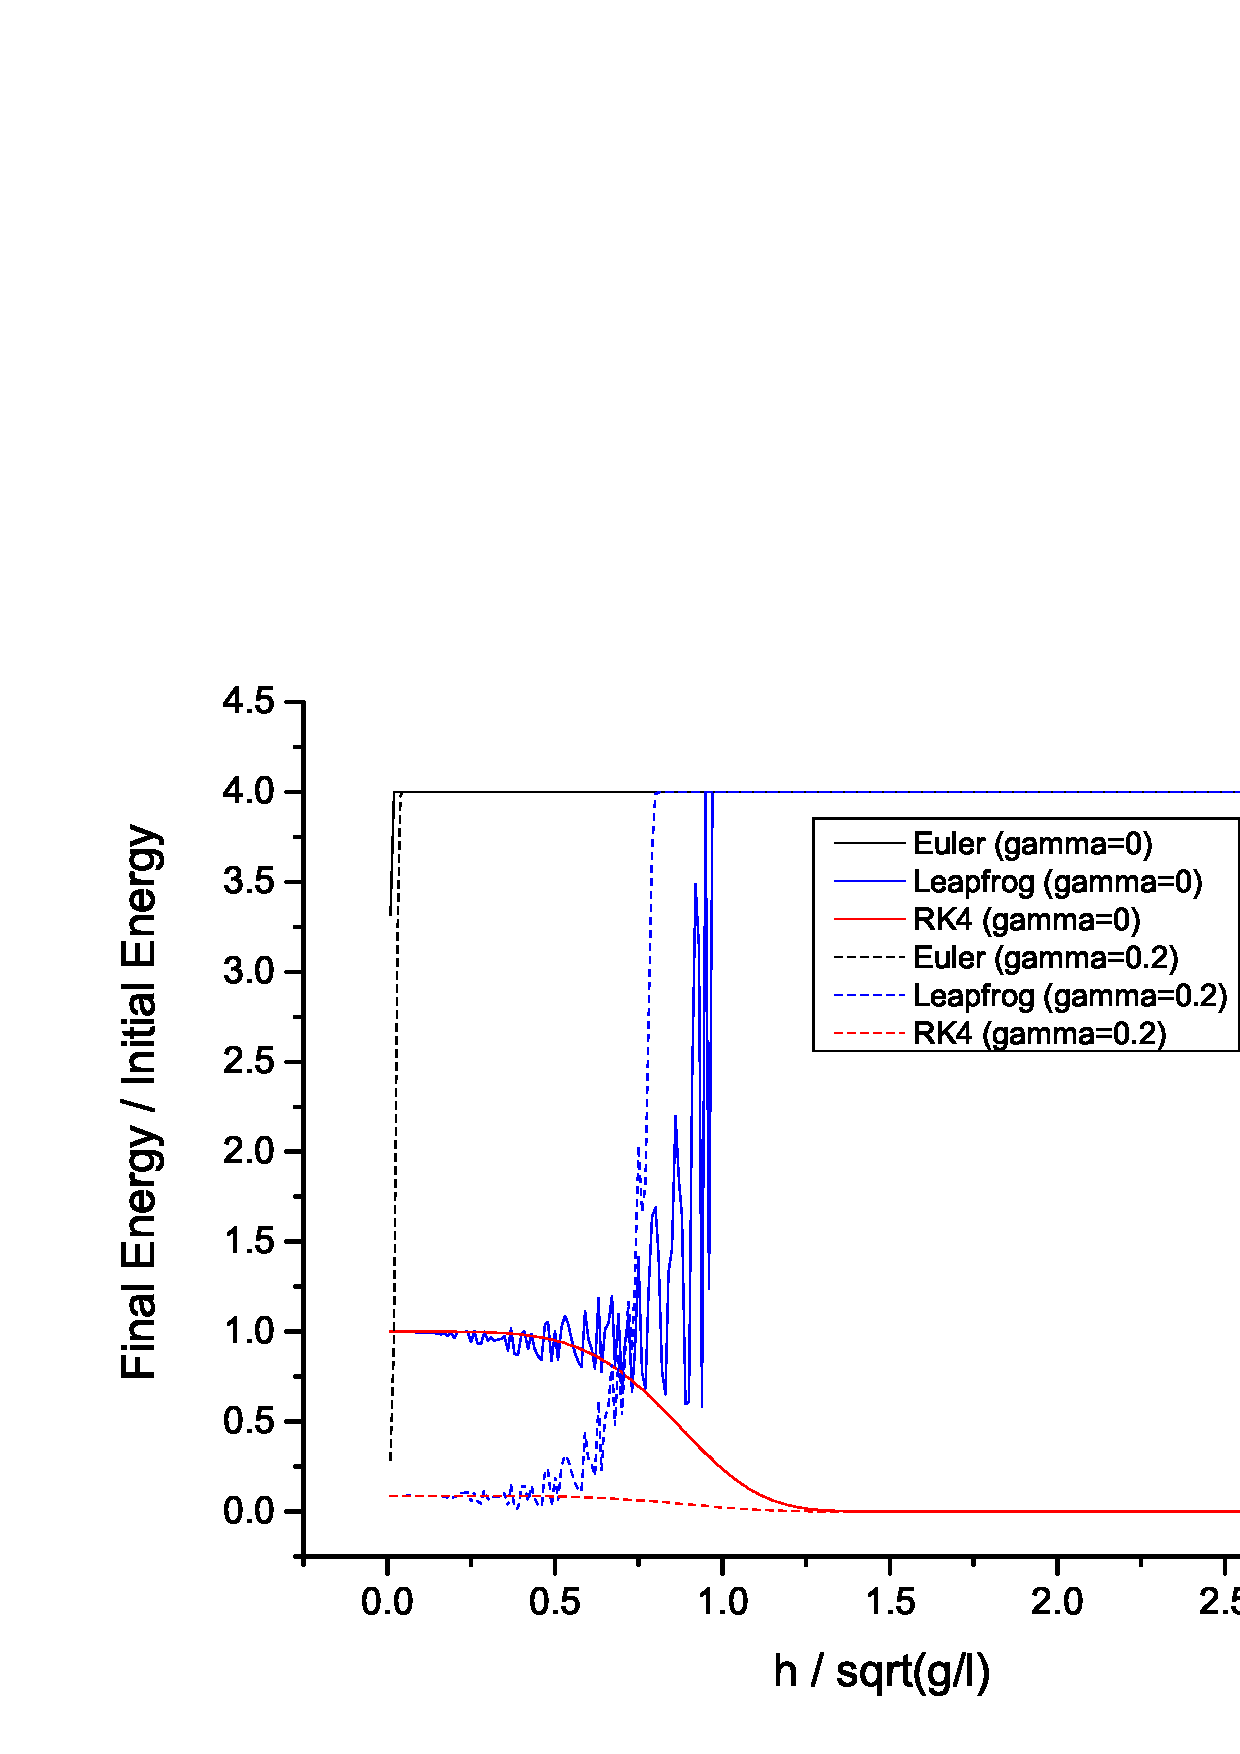
\includegraphics[width=1.1\textwidth]{img/energy_ratio_vs_h.png}
	\caption{The ratio of final pendulum energy ($E$ = kinetic + potential) and intial $E$ versus the step size $h$ for the three numerical methods in the undamped case and a lightly damped case ($\beta$ = 0.2).}
	\label{fig:e_vs_h}
\end{figure}

The results of the stability analysis are summarised in table \ref{tab:sp_stabililty}.

\begin{table}[ht] \label{tab:sp_stability}
	\centering
	\begin{tabular}{ l l l }
		Method & $\beta$ = 0 & $\beta$ = 0.2 \\ \hline
		Euler & \text{unstable} & $h$ = 0.02 \\
		Leapfrog & $h$ = 0.35 & \text{unstable} \\
		RK4 & $h$ = 2.79 & $h$ = 2.81
	\end{tabular}
	\caption{The limit of stability for each method (for cases where the methods provide stable solutions)} % title of Table
\end{table}

\begin{comment}

         88                         88          88                                                   
         88                         88          88                                                   
         88                         88          88                                                   
 ,adPPYb,88  ,adPPYba,  88       88 88,dPPYba,  88  ,adPPYba,    8b,dPPYba,   ,adPPYba, 8b,dPPYba,   
a8"    `Y88 a8"     "8a 88       88 88P'    "8a 88 a8P_____88    88P'    "8a a8P_____88 88P'   `"8a  
8b       88 8b       d8 88       88 88       d8 88 8PP"""""""    88       d8 8PP""""""" 88       88  
"8a,   ,d88 "8a,   ,a8" "8a,   ,a88 88b,   ,a8" 88 "8b,   ,aa    88b,   ,a8" "8b,   ,aa 88       88  
 `"8bbdP"Y8  `"YbbdP"'   `"YbbdP'Y8 8Y"Ybbd8"'  88  `"Ybbd8"'    88`YbbdP"'   `"Ybbd8"' 88       88  
                                                                 88                                  
                                                                 88 
\end{comment}
\section{The Double Pendulum}
\subsection{Theory}
\subsubsection*{System Description \& Parameters}
The idealised double pendulum system comprises the single pendulum setup as before with an added bob of mass $M$ attached by a massless rod (also of length $l$) to the first mass which draws an angle from the vertical of $\psi$ as depicted in figure \ref{fig:pendulum_diag} (b).

\subsubsection*{Equations of Motion}

The mathematics of this system are greatly simplified by choosing constants to take the values set out in equation set \ref{eq:dp_consts}.

\begin{equation} \label{eq:dp_consts}
	R = \frac{M}{m} \;\;\; \text{and} \;\;\; G = \frac{\gamma}{m \sqrt{gl}}
\end{equation}

In terms of these constants, the equations of motion can be expressed as a series of four coupled liner equations, presented as equation \ref{eq:dp_eom}.

\begin{equation}\label{eq:dp_eom}	
\frac{d}{dt} \begin{pmatrix} \theta \\ \phi \\ \omega \\ \nu \end{pmatrix} = 
	\begin{pmatrix}
		0 & 0 & 1 & 0 \\
		0 & 0 & 0 & 1 \\
		-(R+1) & R & -G & 0 \\
		(R+1) & -(R+1) & G(1-R^{-1}) & -G/R
	\end{pmatrix}
	\begin{pmatrix} \theta \\ \phi \\ \omega \\ \nu \end{pmatrix}
\end{equation}

\subsubsection*{A Computer Model for the Single Pendulum System}

From the conclusions of the single pendulum investigation, the forth order Runge-Kutta method was selected to model the double pendulum system. Equation set \ref{eq:rk4_vector} are equally applicable for this scenario taking

\begin{equation} \nonumber
\begin{centering}
\uuline{L} = \begin{pmatrix}
		0 & 0 & 1 & 0 \\
		0 & 0 & 0 & 1 \\
		-(R+1) & R & -G & 0 \\
		(R+1) & -(R+1) & G(1-R^{-1}) & -G/R
	\end{pmatrix} \;\;\; \text{\&} \;\;\; \underline{y}_{n} = \begin{pmatrix} \theta_{n} \\ \phi_{n} \\ \omega_{n} \\ \nu_{n} \end{pmatrix}
\end{centering}
\end{equation}

\subsubsection*{Energy Formulae}
The kinetic and potential energies of the double pendulum are expressed in equations \ref{eq:dp_ke} and \ref{eq:dp_pe} respectively \cite{dp energy formulae}. Both rely on the small angle approximation.

\begin{equation} \label{eq:dp_ke}
T = \frac{1}{2}l^2\left(m\omega^2 + M(\omega^2 + \nu^2) + 2m\nu \right)
\end{equation}

\begin{equation} \label{eq:dp_pe}
U = \frac{1}{2}g\left((m+M)l\theta^2 + Ml\phi^2 \right)
\end{equation}

\subsection{Aims \& Method}
Satisfied with the forth order Runge-Kutta method as a means to reliably model oscillating physical systems computationally, the second investigation focused on the physics of the system being modelled in more detail. Namely, the constants $G$ and $R$ that characterise $\uuline{L}$ for any double pendulum system configuration provided a means to explore how the system acts under a variety of different parameter selections

Throughout all simulations, both pendulum lengths $l$ were kept constant, set equal to $g$ \footnote{$g$ = 9.81 $ms^{-1}$, the acceleratio due to gravity. This value is arbitrary to the dynamics of the system and served only to provide a sanity check to easily identify oscillation periods as multiples of pi as code was debugged}. Each simulation began with $\theta_{initial}$ = 0.1 and $\psi_{initial}$ = 0. Each simulation was run for 100 seconds. A step size of $h$ = 0.01 was used throughout unless explicitly stated otherwise.

To investigate the motion of the pendulums the system was simulated for $R$ values of 0.01, 1.0 and 100 for both the undamped ($G$ = 0) case and the damped case, where $G$ was chosen to equal 1.0. The plots for the pendulum's motion for these configurations are presented in firgures \ref{fig:dp_motion_G0} and \ref{fig:dp_motion_G1}.

%
%	FUCKING DO THIS
%
The individual energies of each pendulum were calculated for each of the aforementioned $R$ and $G$ values to investigate how energy moved through the system. This data is presented in figures \ref{fig:dp_energy_G0} and \ref{fig:dp_energy_G1} included in the appendix to this report.
%
% FUCKING DO THIS
%

%
%	FUCKING DO THIS TOO
%

Lastly, the ratio of final and inital energy was recorded for different values of $R$ as the step size was increased. This allowed for qualitative analysis of the scope of application of the RK4 method for double pendulum systems. Detailed quantitative analysis of the variations exhibited in this dataset are beyond the scope of this investigation. This data is presented in figure \ref{fig:dp_e_vs_h} included in the appendix to this report.
%
% FUCKING DO THIS TOO
%

\subsection{Results \& Discussion}
\subsection*{Motion \& Energy}
% MOTION G=0
Considering first the undamped $G$ = 0 solutions, figure \ref{fig:dp_R0.01_G0} shows that for a higher mass much larger than a lower mass the small oscillation of the upper pendulum drives a much larger oscillation in the lower. The upper pendulum accounts for the majority of the potential energy of the system throughout. As such, when the heavier mass's swinging slows, the lower mass must oscialate much more rapidly to conserve total energy by increasing its kinetic energy.
%%%%%%%%%%%%%%%	assess inclusion of this sentence - did you put those graphs in the appendix?
This energy transfer is depicted graphically in firgure \ref{fig:dp_energy_G0} which can be found in the appendix.

For $R$ = 0, the masses could be said to oscillate \'equally\'; that is to say while the upper oscillation drives the lower to an extent, the amplitudes are within an order of magnitude.
%%%%%%%%%%%%%%%%%% make a comment about energycos this comment is shit otherwise %%%%%%%%%%%%%%%%%%%

For $R$ = 100 in the undamped case, the oscillations of the upper pendulum have much less impact on the motion of the lower mass. The upper mass's amplitude remains effectively constant and its position in space at any one time is strongly determined by the much slower oscillation of the lower, heavier bob which applies a sinusoidal envelope to the upper amsses oscillation.
%%%%%%%%%%%%%%%%%%%% ENERGY %%%%%%%%%%%%%%%%% & REF A FIG

% MOTION G=1
Turning to the damped case, setting $G$ = 1 for an $R$ value of 0.01 we see no oscillation at all. The top, more massive, pendulum is over damped and takes a short time to come to rest in its equilibrium position ($\theta$ = 0). Figure \ref{fig:dp_R0.01_G1} shows how the lower mass takes a much longer amount of time to reach its equilibrium position ($\phi$ = 0). This is best described by imagining the pivot connecting the upper mass to the lower rod as being frictionless while the upper pendulum reaches equilibrium and not frictionless (ie damped) thereafter. This is obviously a departure from the physics we intended to model and shows our small angle approximations have broken down for this configuration.

With $R$ = $G$ = 1 the upper pendulum acts much the same as for the $R$ = 0.01 case, coming to rest at its equilibrium position. The second pendulum behaves more inline with our expectations, coming to rest at its equilibrium poistion much quicker than before without oscillation. It is clear that both pendulums are over damped in this configuration.

Lastly, with $R$ = 100 both pendulums are underdamped. The slow oscillation of the lower pendulum defines a gradually diminishing envelope for the upper pedulum to oscillate within. Eventually the tension caused by the larger lower mass forces the upper pendulum to swing in unison with the lower one. This is observed by the coming together of the two lines, $\theta$ and $\phi$, in \ref{fig:dp_R100_G1} from approximately 10 seconds onwards.

\subsubsection*{Qualitative Stability Analysis for the Double Pendulum}
% ENERGY RATIO VS H FOR DIFFERING R
As for the single pendulum, the undamped double pendulum system was simulated for 100 seconds for different values of $R$. For each value the simulation was run with a step size 0.01 \textless $h$ \textless 4.0 in increments of 0.01. Figure \ref{fig:dp_e_vs_h} (included in the appendix) shows the step size at which the model becomes unstable for each system configuration. There is an obvious trend in the data which reveals that the model can tolerate larger $h$ values provided $R$ is suitably small, ie provided the top mass is suitably larger than the bottom one.

This is because when $R \ll 1$, the overwhelming majority of the system's energy is accounted for by the top mass which and we only need to model a simple single pendulum to attain sensible, stable energy values. Conversely, for $R \gg 1$, the bottom pendulum must be well modelled by the simulation to produce stable energy values. As this system is more complex than a single pendulum and beyond the scope of application of our small angle RK4 method, the simulation soon becomes unstable.

\begin{figure}[h!] \label{fig:dp_motion_G0}
  \centering
  \begin{subfigure}[h]{0.5\textwidth}
    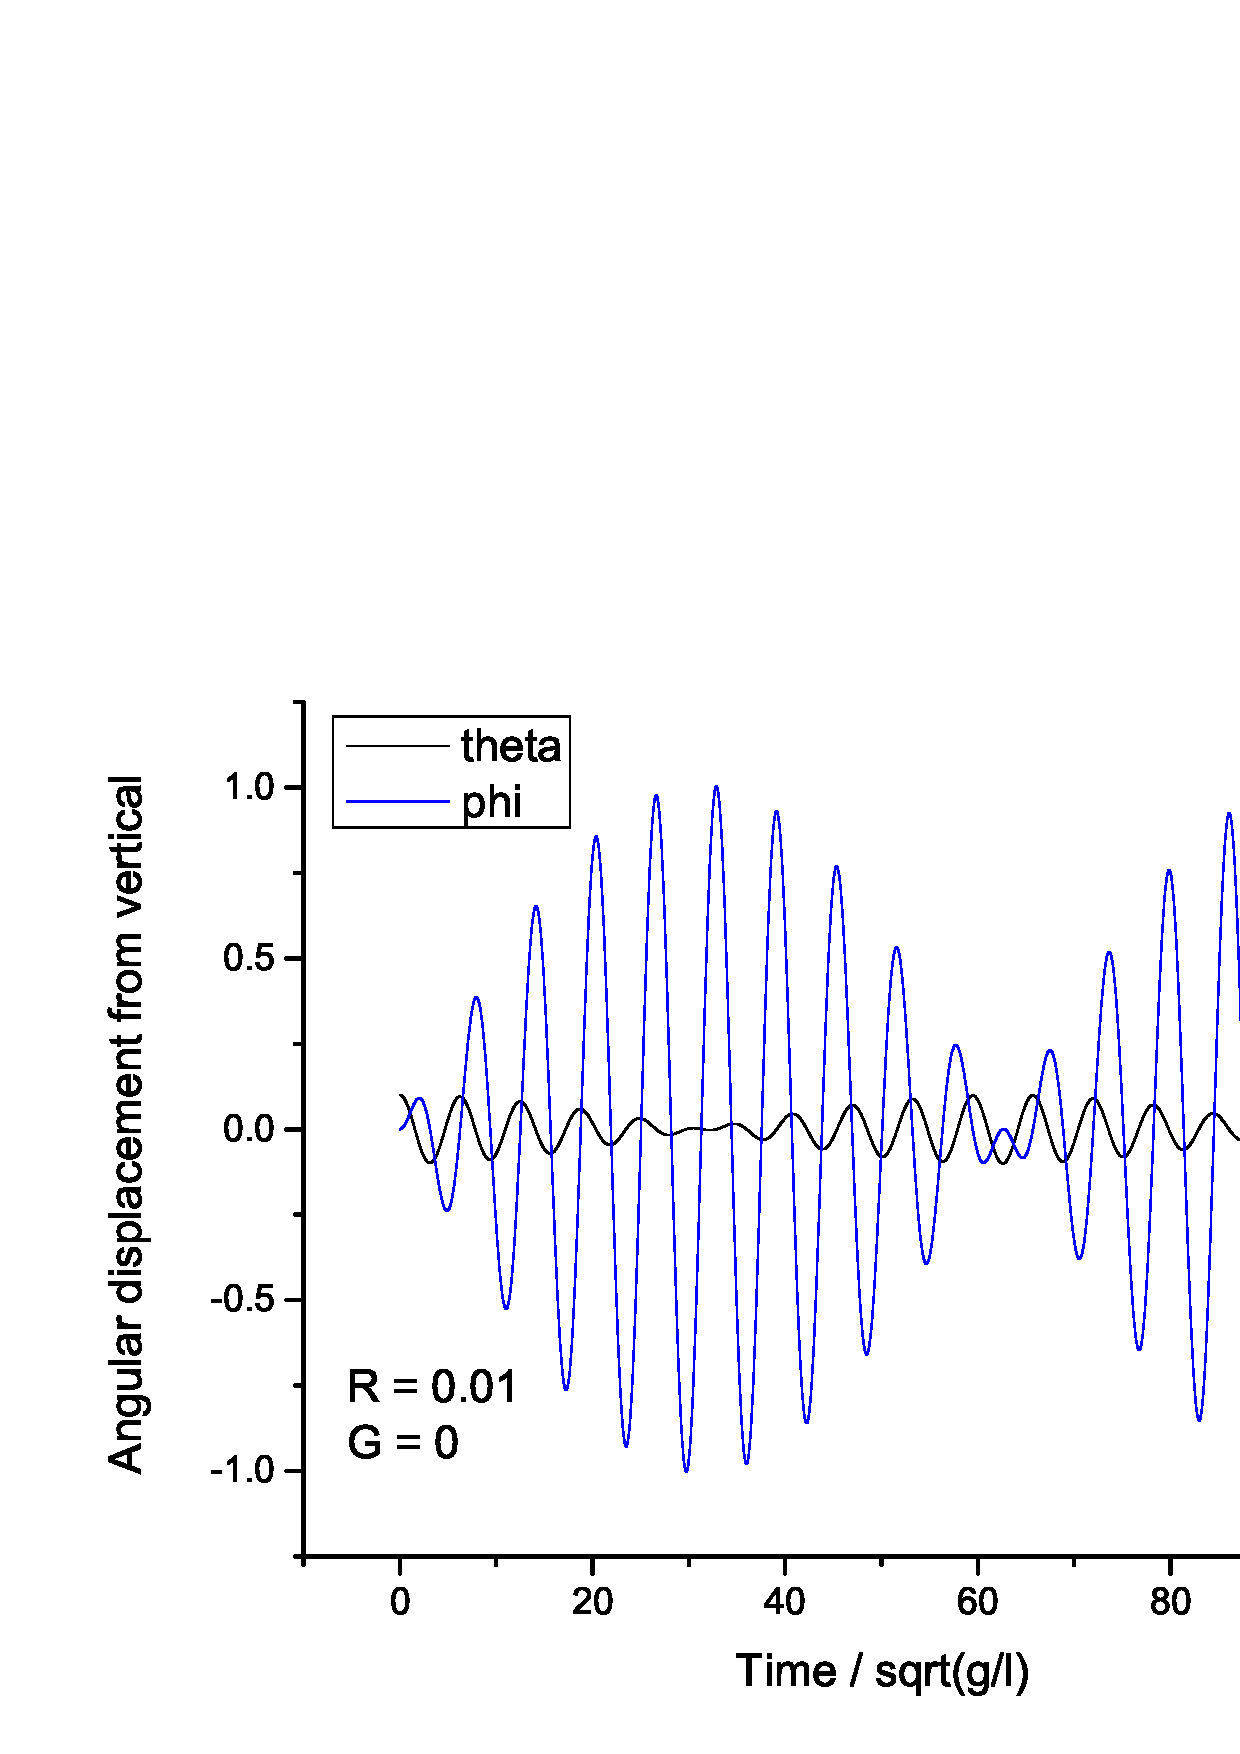
\includegraphics[width=\textwidth]{img/dp/R=0-01_G=0.png}
    \captionsetup{width=0.85\textwidth}
    \caption{$R$ = 0.01, $G$ = 0}
    \label{fig:dp_R0.01_G0}
  \end{subfigure}%
  ~ %add desired spacing between images, e. g. ~, \quad, \qquad etc.
  \begin{subfigure}[h]{0.5\textwidth}
    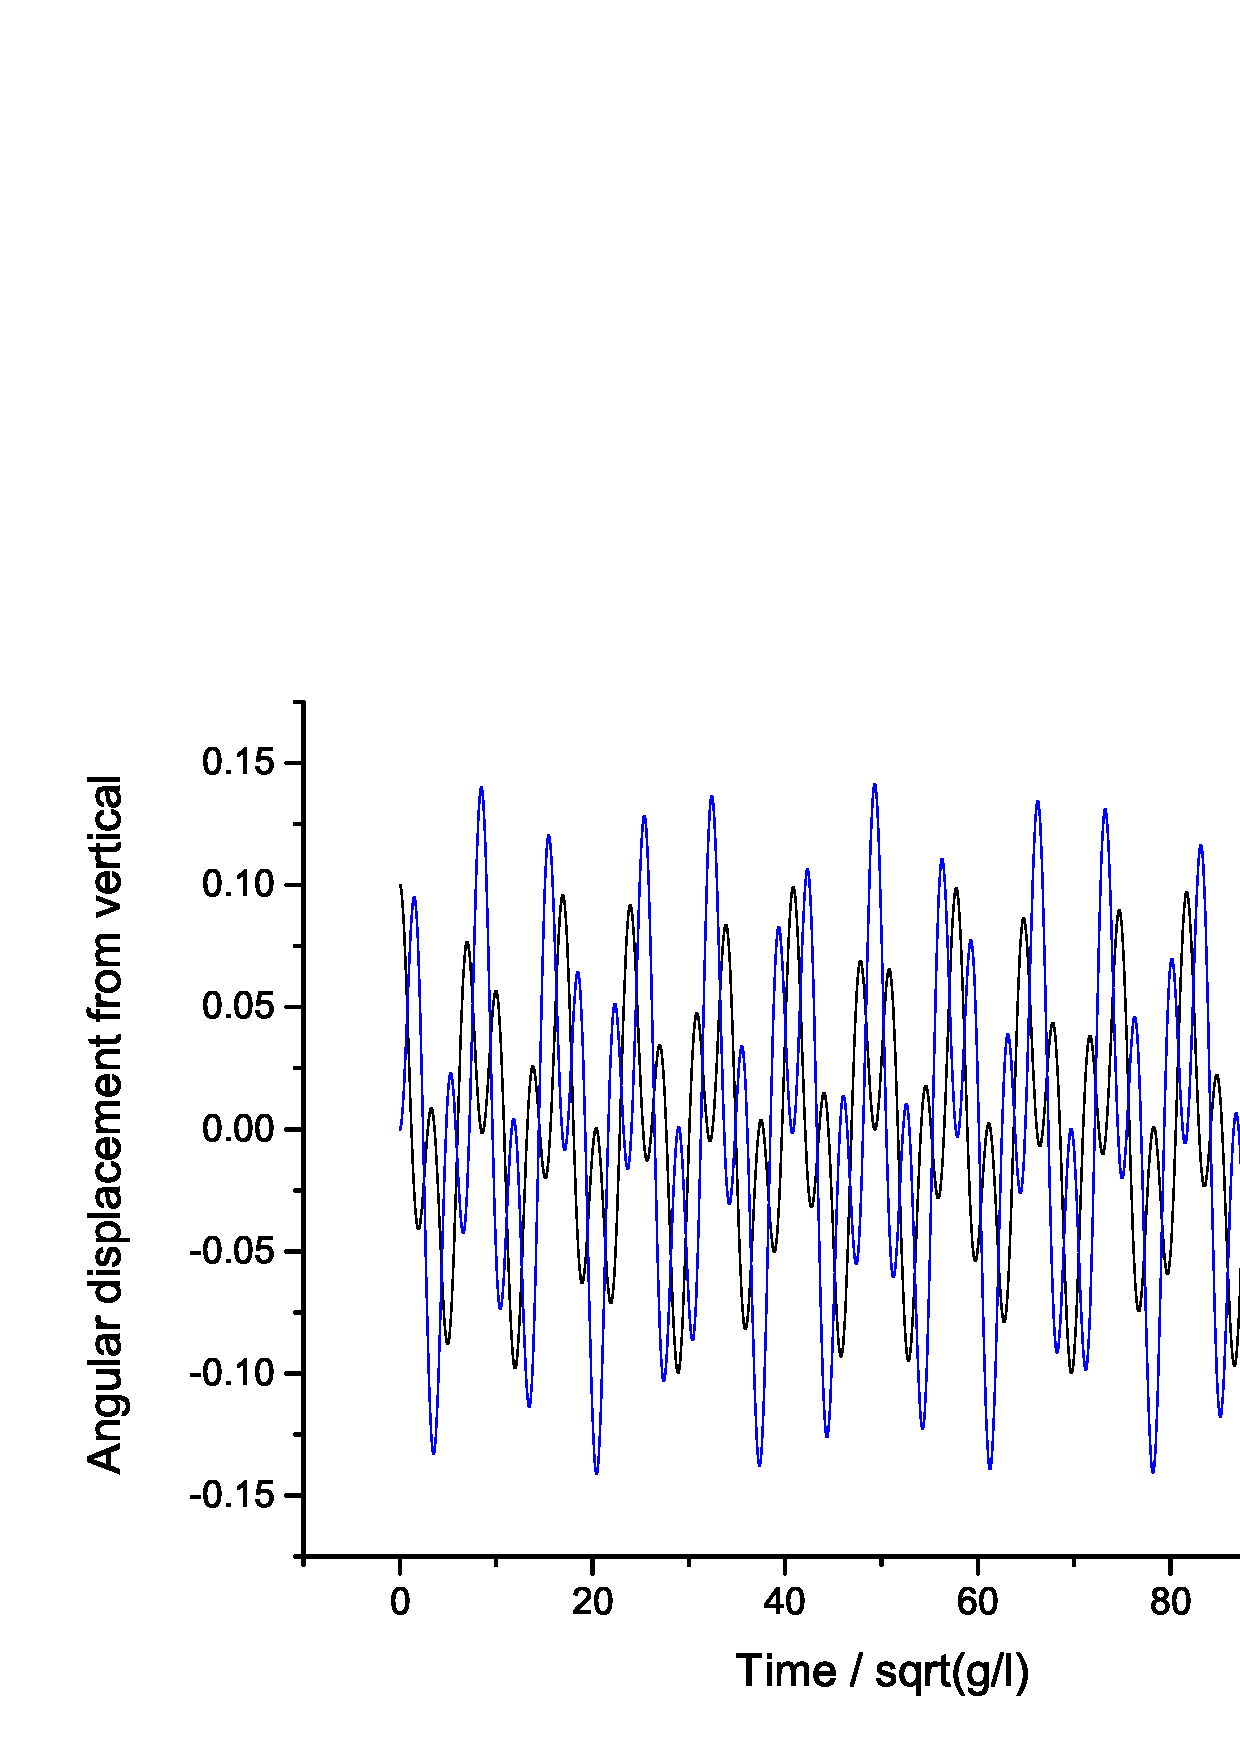
\includegraphics[width=\textwidth]{img/dp/R=1_G=0.png}
    \captionsetup{width=0.85\textwidth}
    \caption{$R$ = 1, $G$ = 0}
    \label{fig:dp_R1_G0}
  \end{subfigure}
  ~ %add desired spacing between images, e. g. ~, \quad, \qquad etc.
  \begin{subfigure}[h]{0.5\textwidth}
    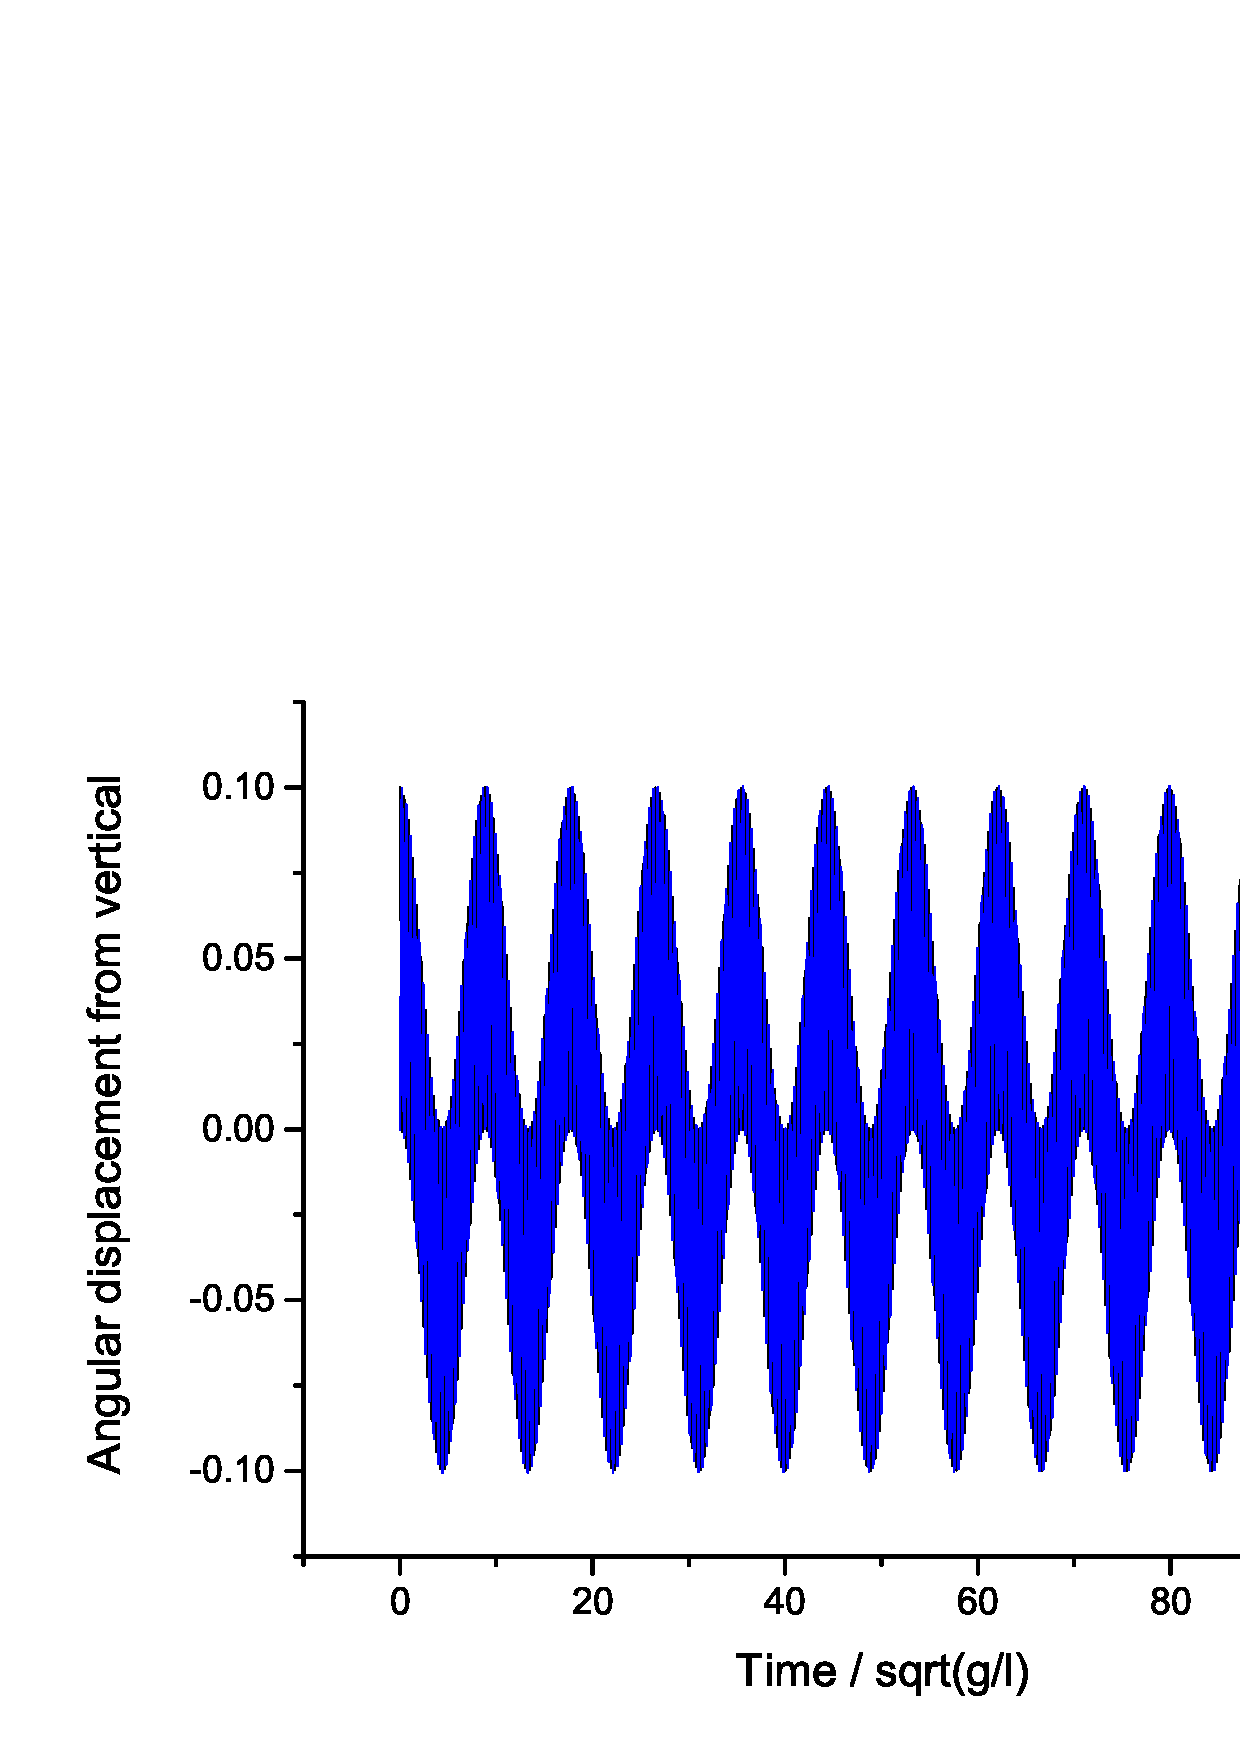
\includegraphics[width=\textwidth]{img/dp/R=100_G=0.png}
    \captionsetup{width=0.85\textwidth}
    \caption{$R$ = 100, $G$ = 0}
    \label{fig:dp_R1_G0}
  \end{subfigure}
  \caption{The motion of the double pendulum system for different mass ratios ($R$ values) in the undamped case ($G$ = 0)}
\end{figure}

\begin{figure}[h!] \label{fig:dp_motion_G1}
  \centering
  \begin{subfigure}[h]{0.5\textwidth}
    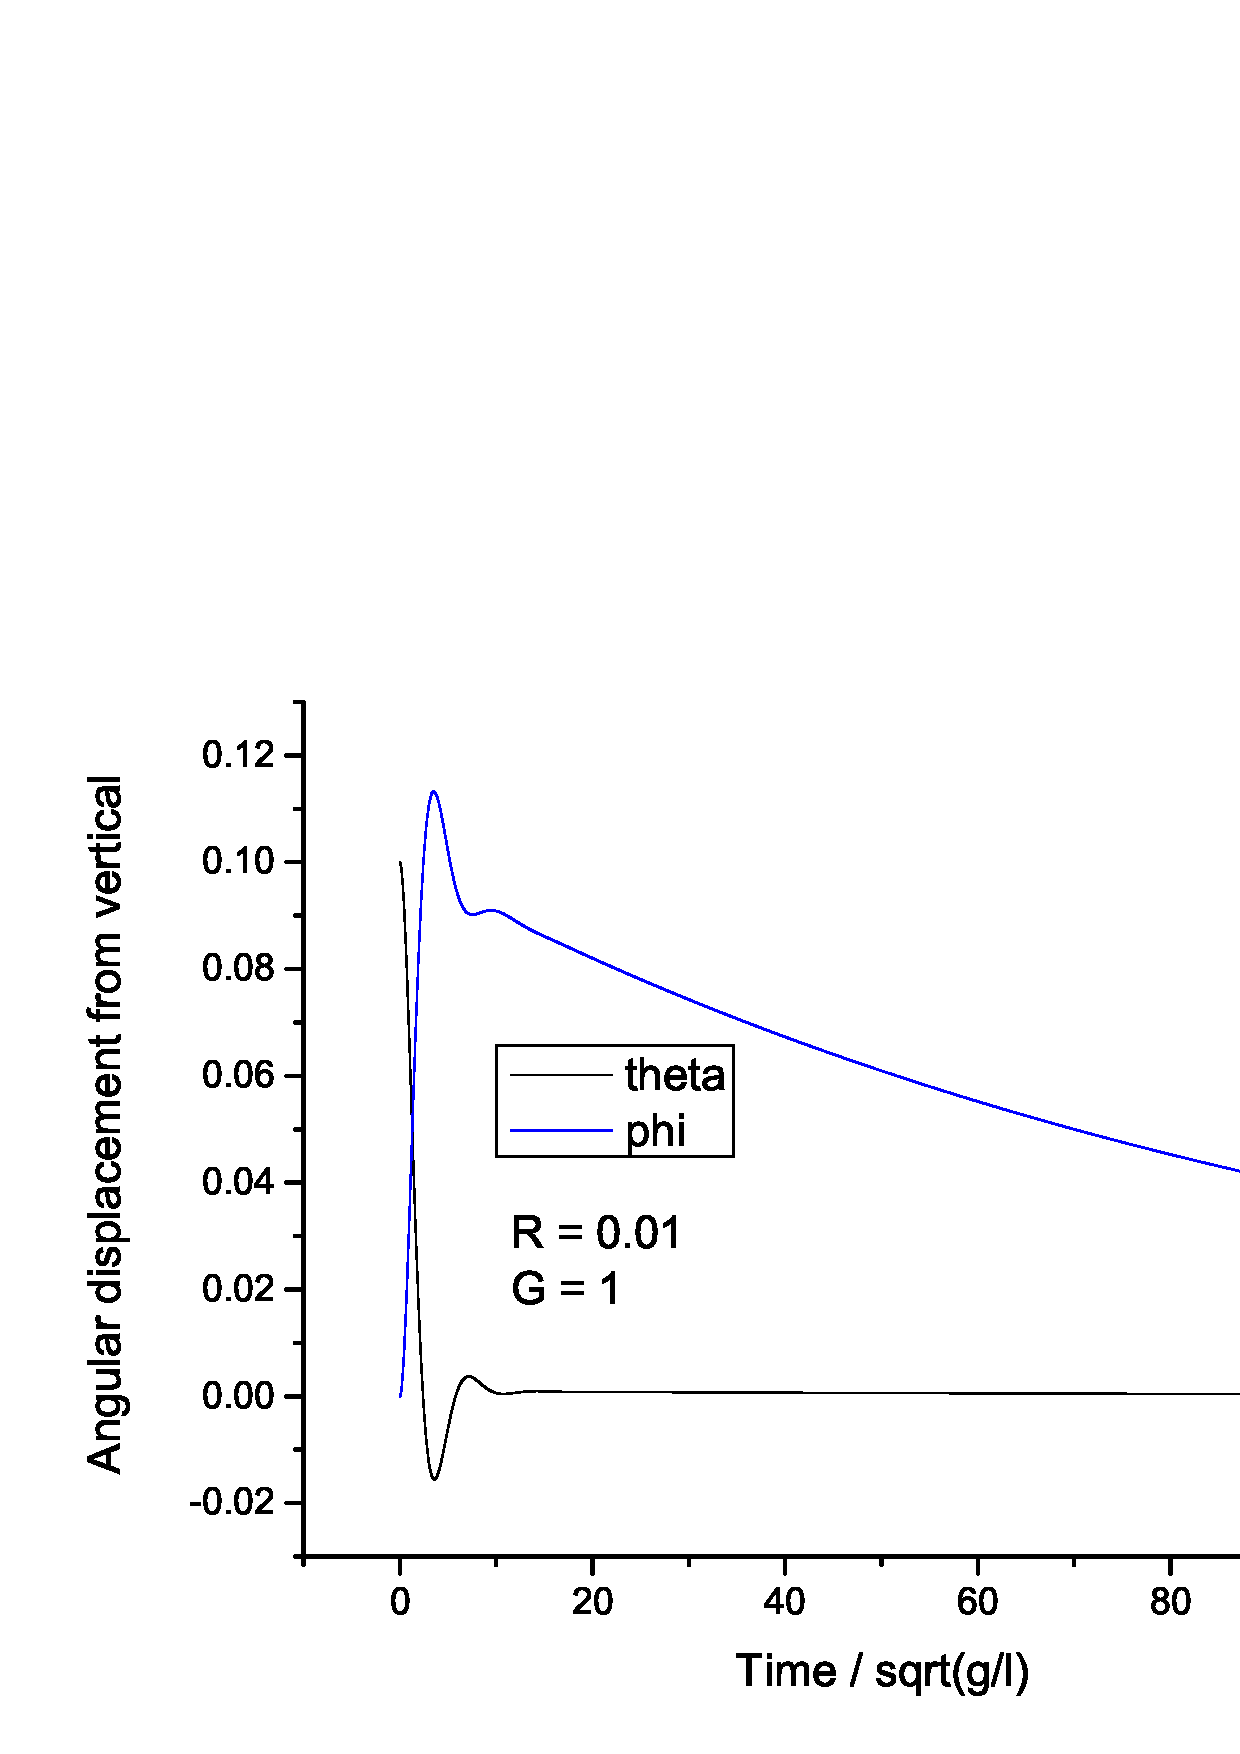
\includegraphics[width=\textwidth]{img/dp/R=0-01_G=1.png}
    \captionsetup{width=0.85\textwidth}
    \caption{$R$ = 0.01, $G$ = 1}
    \label{fig:dp_R0.01_G0}
  \end{subfigure}%
  ~ %add desired spacing between images, e. g. ~, \quad, \qquad etc.
  \begin{subfigure}[h]{0.5\textwidth}
    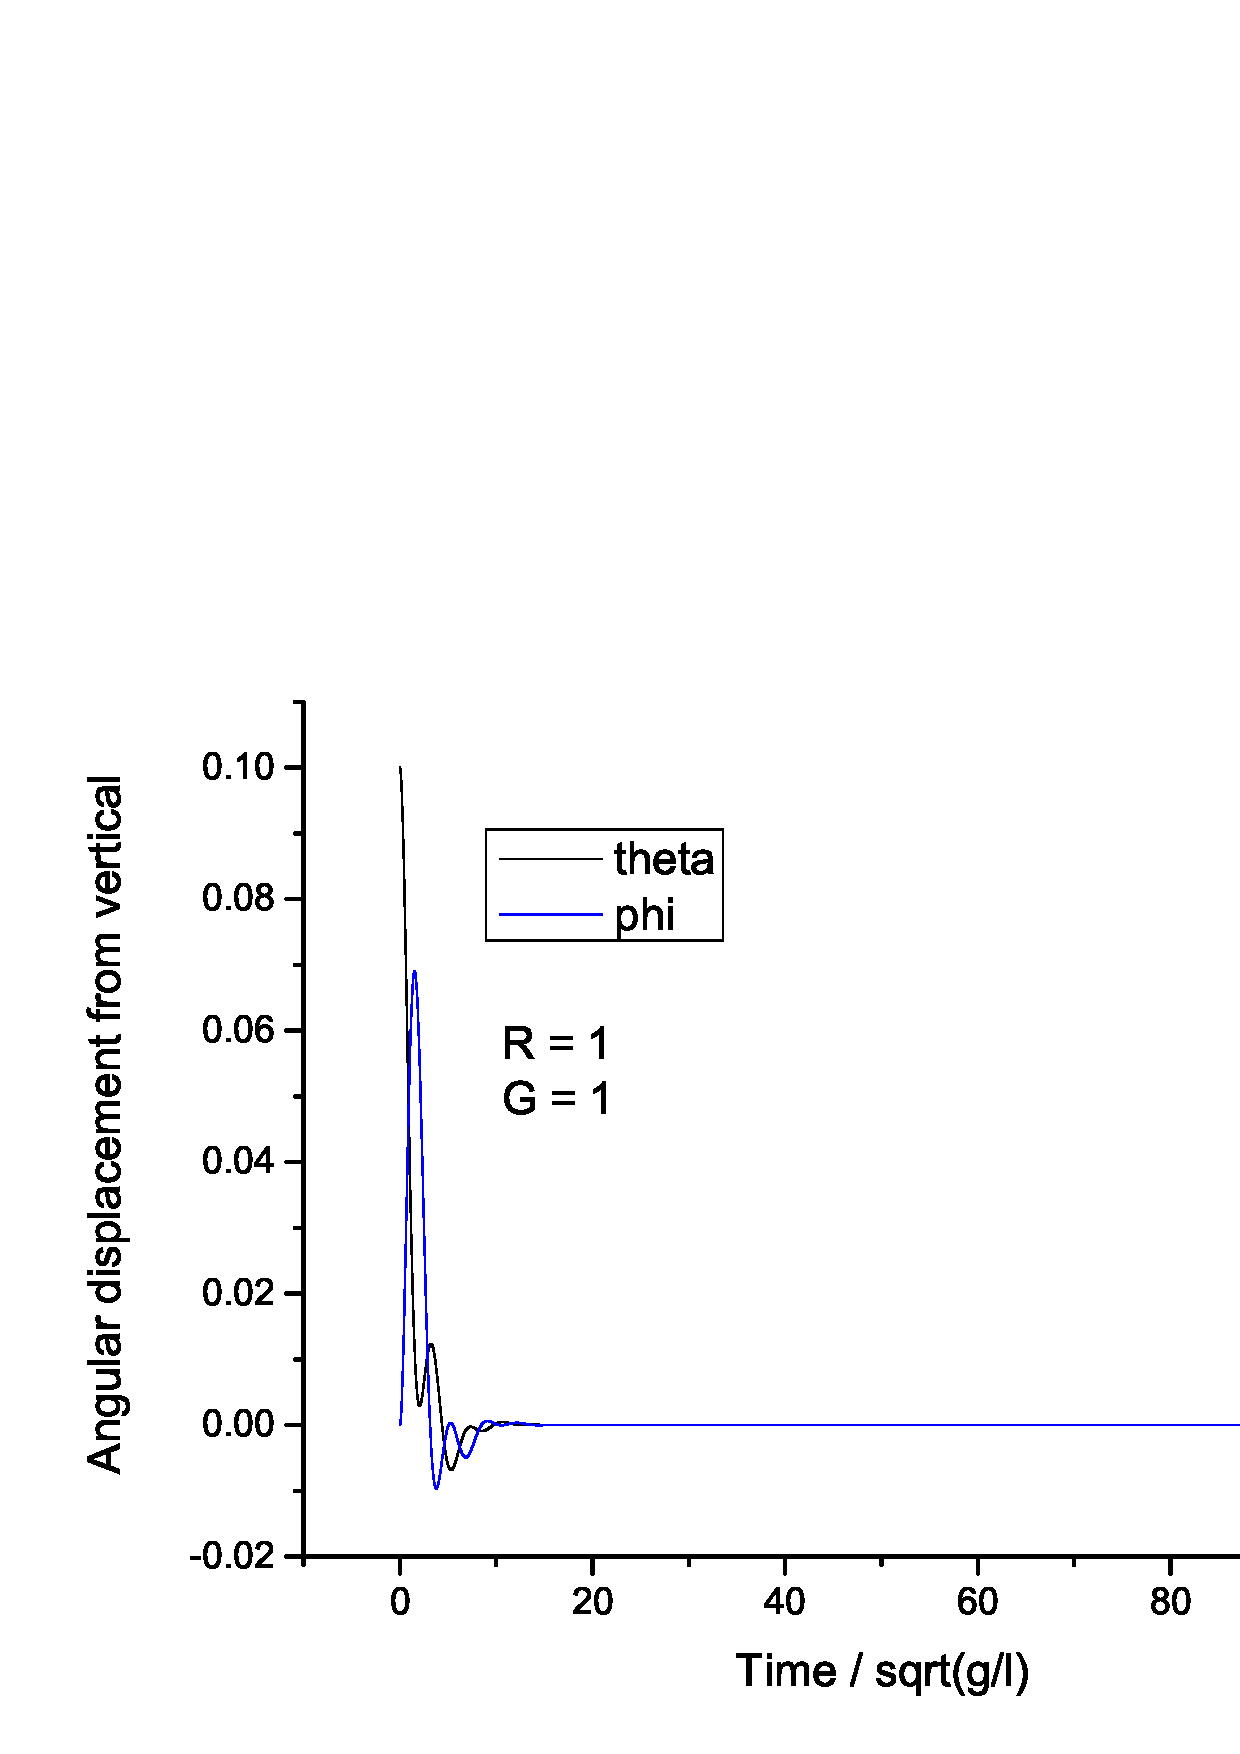
\includegraphics[width=\textwidth]{img/dp/R=1_G=1.png}
    \captionsetup{width=0.85\textwidth}
    \caption{$R$ = 1, $G$ = 1}
    \label{fig:dp_R1_G0}
  \end{subfigure}
  ~ %add desired spacing between images, e. g. ~, \quad, \qquad etc.
  \begin{subfigure}[h]{0.5\textwidth}
    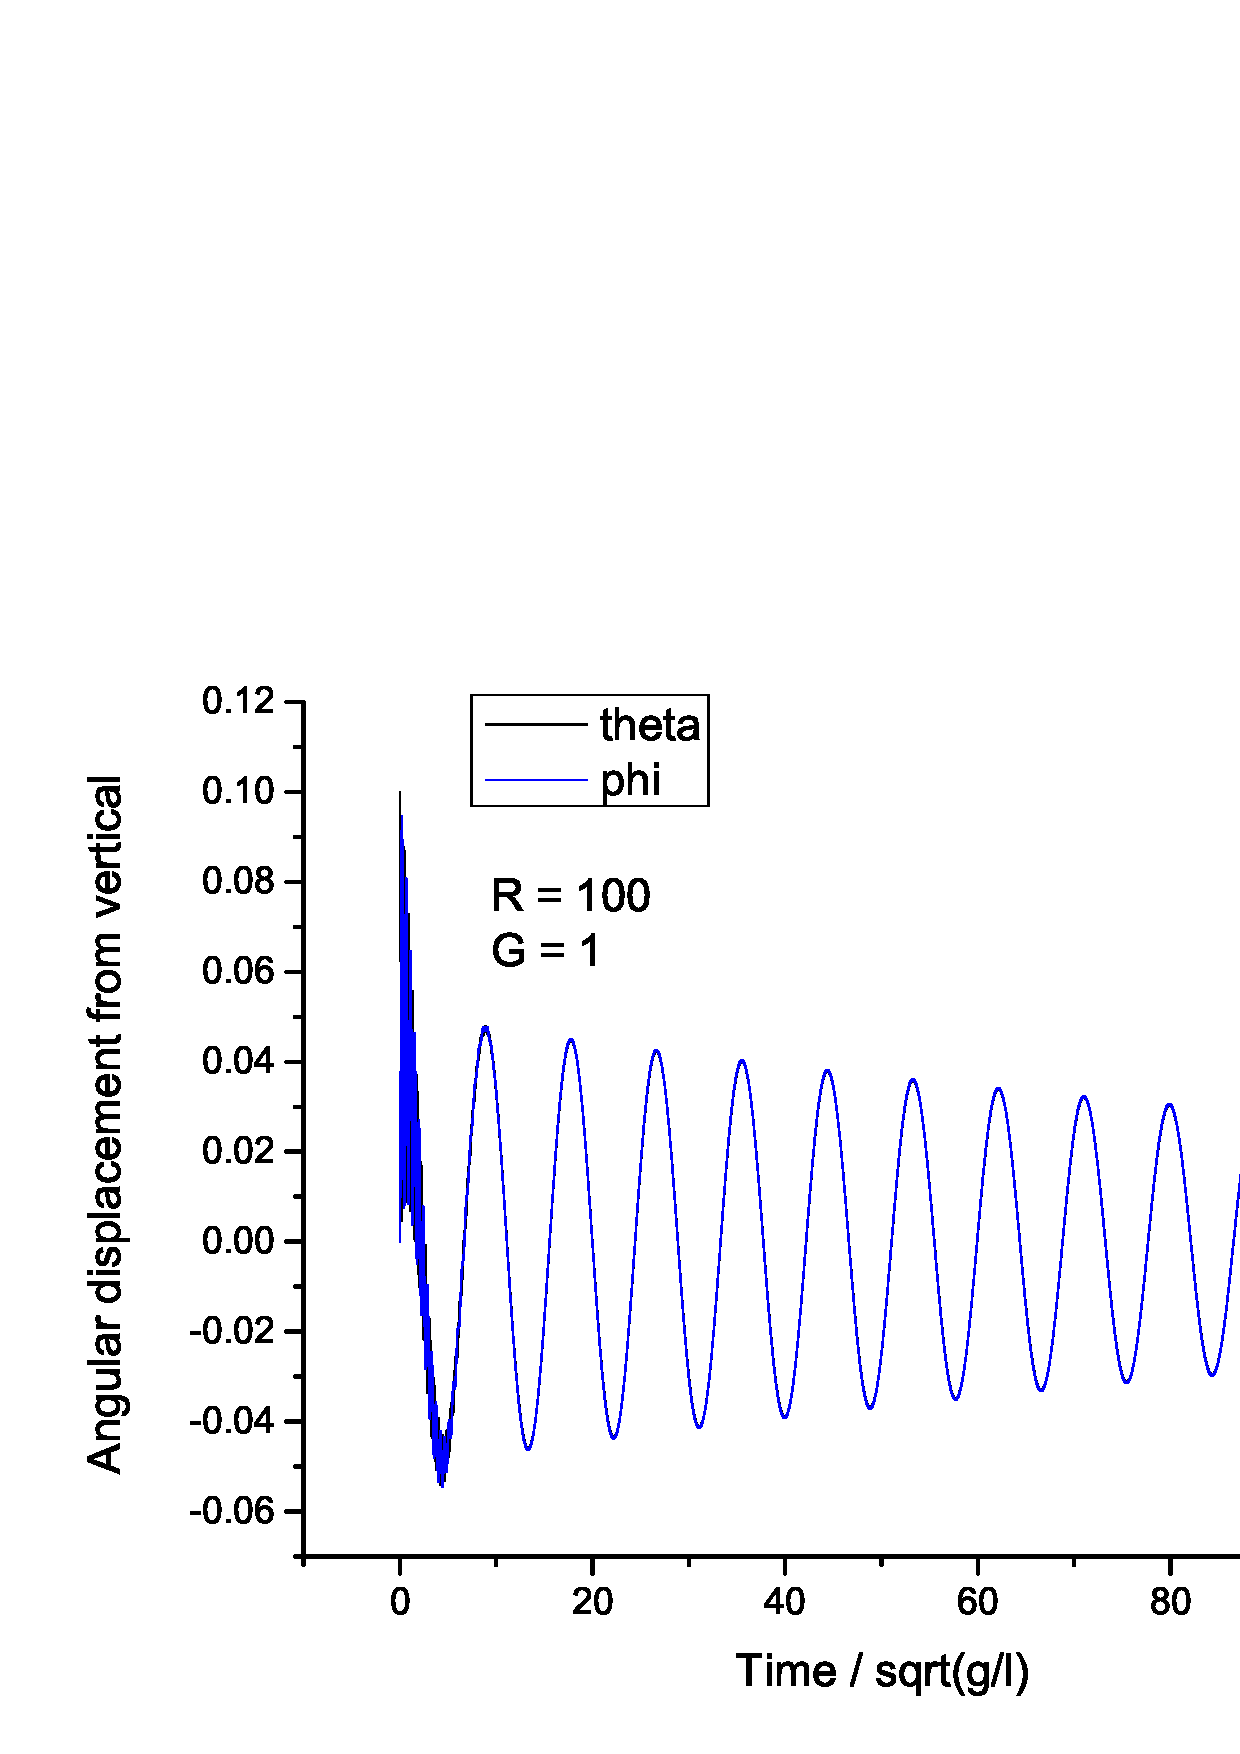
\includegraphics[width=\textwidth]{img/dp/R=100_G=1.png}
    \captionsetup{width=0.85\textwidth}
    \caption{$R$ = 100, $G$ = 1}
    \label{fig:dp_R1_G0}
  \end{subfigure}
  \caption{The motion of the double pendulum system for different mass ratios ($R$ values) in the damped case ($G$ = 1)}
\end{figure}

%
%	COULD JUST GO IN CONCLUSION
%
% A FURTHER AVENUE OF INVESTIGATION IS WHAT HAPPENS TO LEAPFROG AS OSCILLATION AMP. APPROACHES ZERO
% WHAT PARAMETERS WOULD BE REQUIRED FOR IT TO PRODUCE MORE STABLE RESULTS?
%
\section{Conclusion}
A single pendulum system was first modelled using three different numerical methods, Euler's method, Leapfrog and fourth order Runge-Kutta. Following a stability analysis of these three computational models RK4 was selected as the most appropriate method to model an idealised double pendulum system due to its stable results at large step sizes and applicability to both damped and undamped oscillationg systems.

The motion and energy dynamics of the double pendulum system were investigated next and an understanding of the dynamics of this system was derived from the output of the computational models. Sanity checking results against what common sense would predict allowed us to identify points where our computational model broke down. This model was shown to produce more stable results for smaller ratios of top-to-bottom mass in the undamped case through stability analysis.

Through the course of this project certain further avenues of investigation. The curves in figure \ref{fig:dp_e_vs_h} exhibited a curious tendency to an energy ratio of $\frac{1}{2}$ before becoming unstable and the leapfrog method in the time region where oscillations approach zero and its solutions become unstable both present interesting phenomena beyond the scope of this report.

\newpage
\section{Appendix} \label{app:Appendix}

\begin{comment}

\begin{figure}[h!] \label{fig:dp_energy_G0}
	\vspace{-50pt}
  \centering
  \begin{subfigure}[h]{0.7\textwidth}
    \includegraphics[width=\textwidth]{img/dp/e_R=0-01_G=1.png}
    \captionsetup{width=0.85\textwidth}
    \caption{$R$ = 0.01, $G$ = 1}
    \label{fig:dp_e_R0.01_G0}
  \end{subfigure}%
  \\ %add desired spacing between images, e. g. ~, \quad, \qquad etc.
  \begin{subfigure}[h]{0.7\textwidth}
    \includegraphics[width=\textwidth]{img/dp/e_R=1_G=1.png}
    \captionsetup{width=0.85\textwidth}
    \caption{$R$ = 1, $G$ = 1}
    \label{fig:dp_e_R1_G0}
  \end{subfigure}
  \\ %add desired spacing between images, e. g. ~, \quad, \qquad etc.
  \begin{subfigure}[h]{0.7\textwidth}
    \includegraphics[width=\textwidth]{img/dp/e_R=100_G=1.png}
    \captionsetup{width=0.85\textwidth}
    \caption{$R$ = 100, $G$ = 1}
    \label{fig:dp_e_R1_G0}
  \end{subfigure}
  \caption{OVERALL CAPTION}
\end{figure}

\begin{figure}[h!] \label{fig:dp_energy_G1}
	\vspace{-50pt}
  \centering
  \begin{subfigure}[h]{0.7\textwidth}
    \includegraphics[width=\textwidth]{img/dp/e_R=0-01_G=1.png}
    \captionsetup{width=0.85\textwidth}
    \caption{$R$ = 0.01, $G$ = 1}
    \label{fig:dp_e_R0.01_G0}
  \end{subfigure}%
  \\ %add desired spacing between images, e. g. ~, \quad, \qquad etc.
  \begin{subfigure}[h]{0.7\textwidth}
    \includegraphics[width=\textwidth]{img/dp/e_R=1_G=1.png}
    \captionsetup{width=0.85\textwidth}
    \caption{$R$ = 1, $G$ = 1}
    \label{fig:dp_e_R1_G0}
  \end{subfigure}
  \\ %add desired spacing between images, e. g. ~, \quad, \qquad etc.
  \begin{subfigure}[h]{0.7\textwidth}
    \includegraphics[width=\textwidth]{img/dp/e_R=100_G=1.png}
    \captionsetup{width=0.85\textwidth}
    \caption{$R$ = 100, $G$ = 1}
    \label{fig:dp_e_R1_G0}
  \end{subfigure}
  \caption{OVERALL CAPTION}
\end{figure}

\end{comment}

\newpage

\begin{thebibliography}{10}
\bibitem{dp energy formulae} http://www2.ph.ed.ac.uk/\~egardi/MfP3-Dynamics/Dynamics\_lecture\_16.pdf - Einan Gardi (accessed 10/11/2013)
\end{thebibliography}

\end{document}  